\chapter{Comparison}\label{comparison}
This chapter will compare iTasks and LTasks using a case study of the breakfast example adapted from Naus \cite{naus2020assisting} in listing \ref{lst:clean_breakfast}. To make it into a functioning example with editors, we need to modify it a bit. \lua{makeTea}, \lua{makeCoffee} and \lua{makeSandwich} are here modelled as editors. In the real world, they will be tasks that have no value initially, and a constant value once the tea, coffee or sandwich has been made. This allows us to make use of the standard task combinators without helper functions, like the example in listing \ref{lst:clean_breakfast}. This complete but contrived example is however more interesting because it makes use of editors and the transform combinator. The entire example can be seen in appendix \ref{appendix-breakfast}.

\subsection{Main task and combinators}
The high level overview looks like listing \ref{lst:comparison_breakfast}. As you can see, they are almost identical. Lua uses different operators, and instead of an \clean{OnValue} there is a table with a \lua{fn} field.

\begin{figure}[ht]
\begin{subfigure}{\textwidth}
\centering
\begin{minted}{clean}
((makeTea -||- makeCoffee) -&&- makeSandwich) >>* [OnValue maybeEatBreakfast]
\end{minted}
\caption{In iTasks}
\label{lst:comparison_breakfast_clean}
\end{subfigure}
\begin{subfigure}{\textwidth}
\centering
\bigskip % space between subfigures
\begin{minted}{lua}
((makeTea | makeCoffee) & makeSandwich) .. {{fn = maybeEatBreakfast}}
\end{minted}
\caption{In LTasks}
\label{lst:comparison_breakfast_lua}
\end{subfigure}
\caption{The main part of the breakfast example.}
\label{lst:comparison_breakfast}
\end{figure}

\subsection{Editors}
There is a bit more difference in making editors than the basic combinators. iTasks uses combinators to add hints to editors, while LTasks includes the hints in the function signature, for simplicity. The most important difference in this example comes from the fact that Clean is statically typed, so the transformation function cannot return different types as in Lua. Instead, it has to return a maybe (an algebraic data type).

\begin{figure}[ht]
\begin{subfigure}{\textwidth}
\centering
\begin{minted}{clean}
makeTea = updateInformation [] False <<@ Hint "Make tea?"
        @ (\x -> if x (?Just "Tea") ?None)
        @? tvFromMaybe
\end{minted}
\caption{In iTasks}
\label{lst:comparison_editors_clean}
\end{subfigure}
\begin{subfigure}{\textwidth}
\centering
\bigskip % space between subfigures
\begin{minted}{lua}
local makeTea = editor.editBoolean(false, "make tea?")
    :transformValue(function(x) return x and "Tea" or nil end)
\end{minted}
\caption{In LTasks}
\label{lst:comparison_editors_lua}
\end{subfigure}
\caption{Making a boolean editor that results in either ``Tea'' or nothing.}
\label{lst:comparison_editors}
\end{figure}

\subsection{Helper function}
The wrapping of the actual value in a \clean{TaskValue} and a maybe type is harder to work with, we need to use pattern matching. Listing \ref{lst:comparison_maybe} shows the helper functions that are needed to create a \lua{viewInformation} task only if a food and drink are chosen. These functions are needed due to the fact that this is a contrived example.

\begin{figure}[ht]
\begin{subfigure}{\textwidth}
\centering
% maybeEatBreakfast :: (TaskValue (String, String)) -> ? (Task String)
\begin{minted}{clean}
maybeEatBreakfast (Value (drink, food) _) = ?Just (eatBreakfast drink food)
maybeEatBreakfast _ = ?None
\end{minted}
\caption{In iTasks}
\label{lst:comparison_maybe_clean}
\end{subfigure}
\begin{subfigure}{\textwidth}
\centering
\bigskip % space between subfigures
\begin{minted}{lua}
local function maybeEatBreakfast(value)
    if value[1] ~= nil and value[2] ~= nil then
        return eatBreakfast(value[1], value[2])
    end
end
\end{minted}
\caption{In LTasks}
\label{lst:comparison_maybe_lua}
\end{subfigure}
\caption{Making a boolean editor that results in either "Tea" or nothing.}
\label{lst:comparison_maybe}
\end{figure}

\subsection{User interface}
The user interface for LTasks (shown in figure \ref{fig:comparison_ltask_ui}) is made to serve two purposes: to be the bare minimum for a TOP proof-of-concept, and to make clear that the behaviour is correct for TOP. For that reason, it looks very different to the iTasks UI.

Let us set aside the differences in visual display for now (LTasks uses a textual UI while iTasks uses a webpage). The textual UI of LTasks shows the structure of the task at the top. This is not only useful for seeing that the structure is indeed correct, but also for keeping a mental image of where you are navigated to. This is not necessary in iTasks because it shows everything at once instead of entering sub-menus (fig. \ref{fig:comparison_itask_ui}). iTasks hides the way in which \lua{makeTea} and \lua{makeCoffee} are composed with \lua{makeSandwich}, while the LTasks UI makes this more explicit.

\begin{figure}
\centering
\begin{subfigure}{0.8\textwidth}
    \centering
    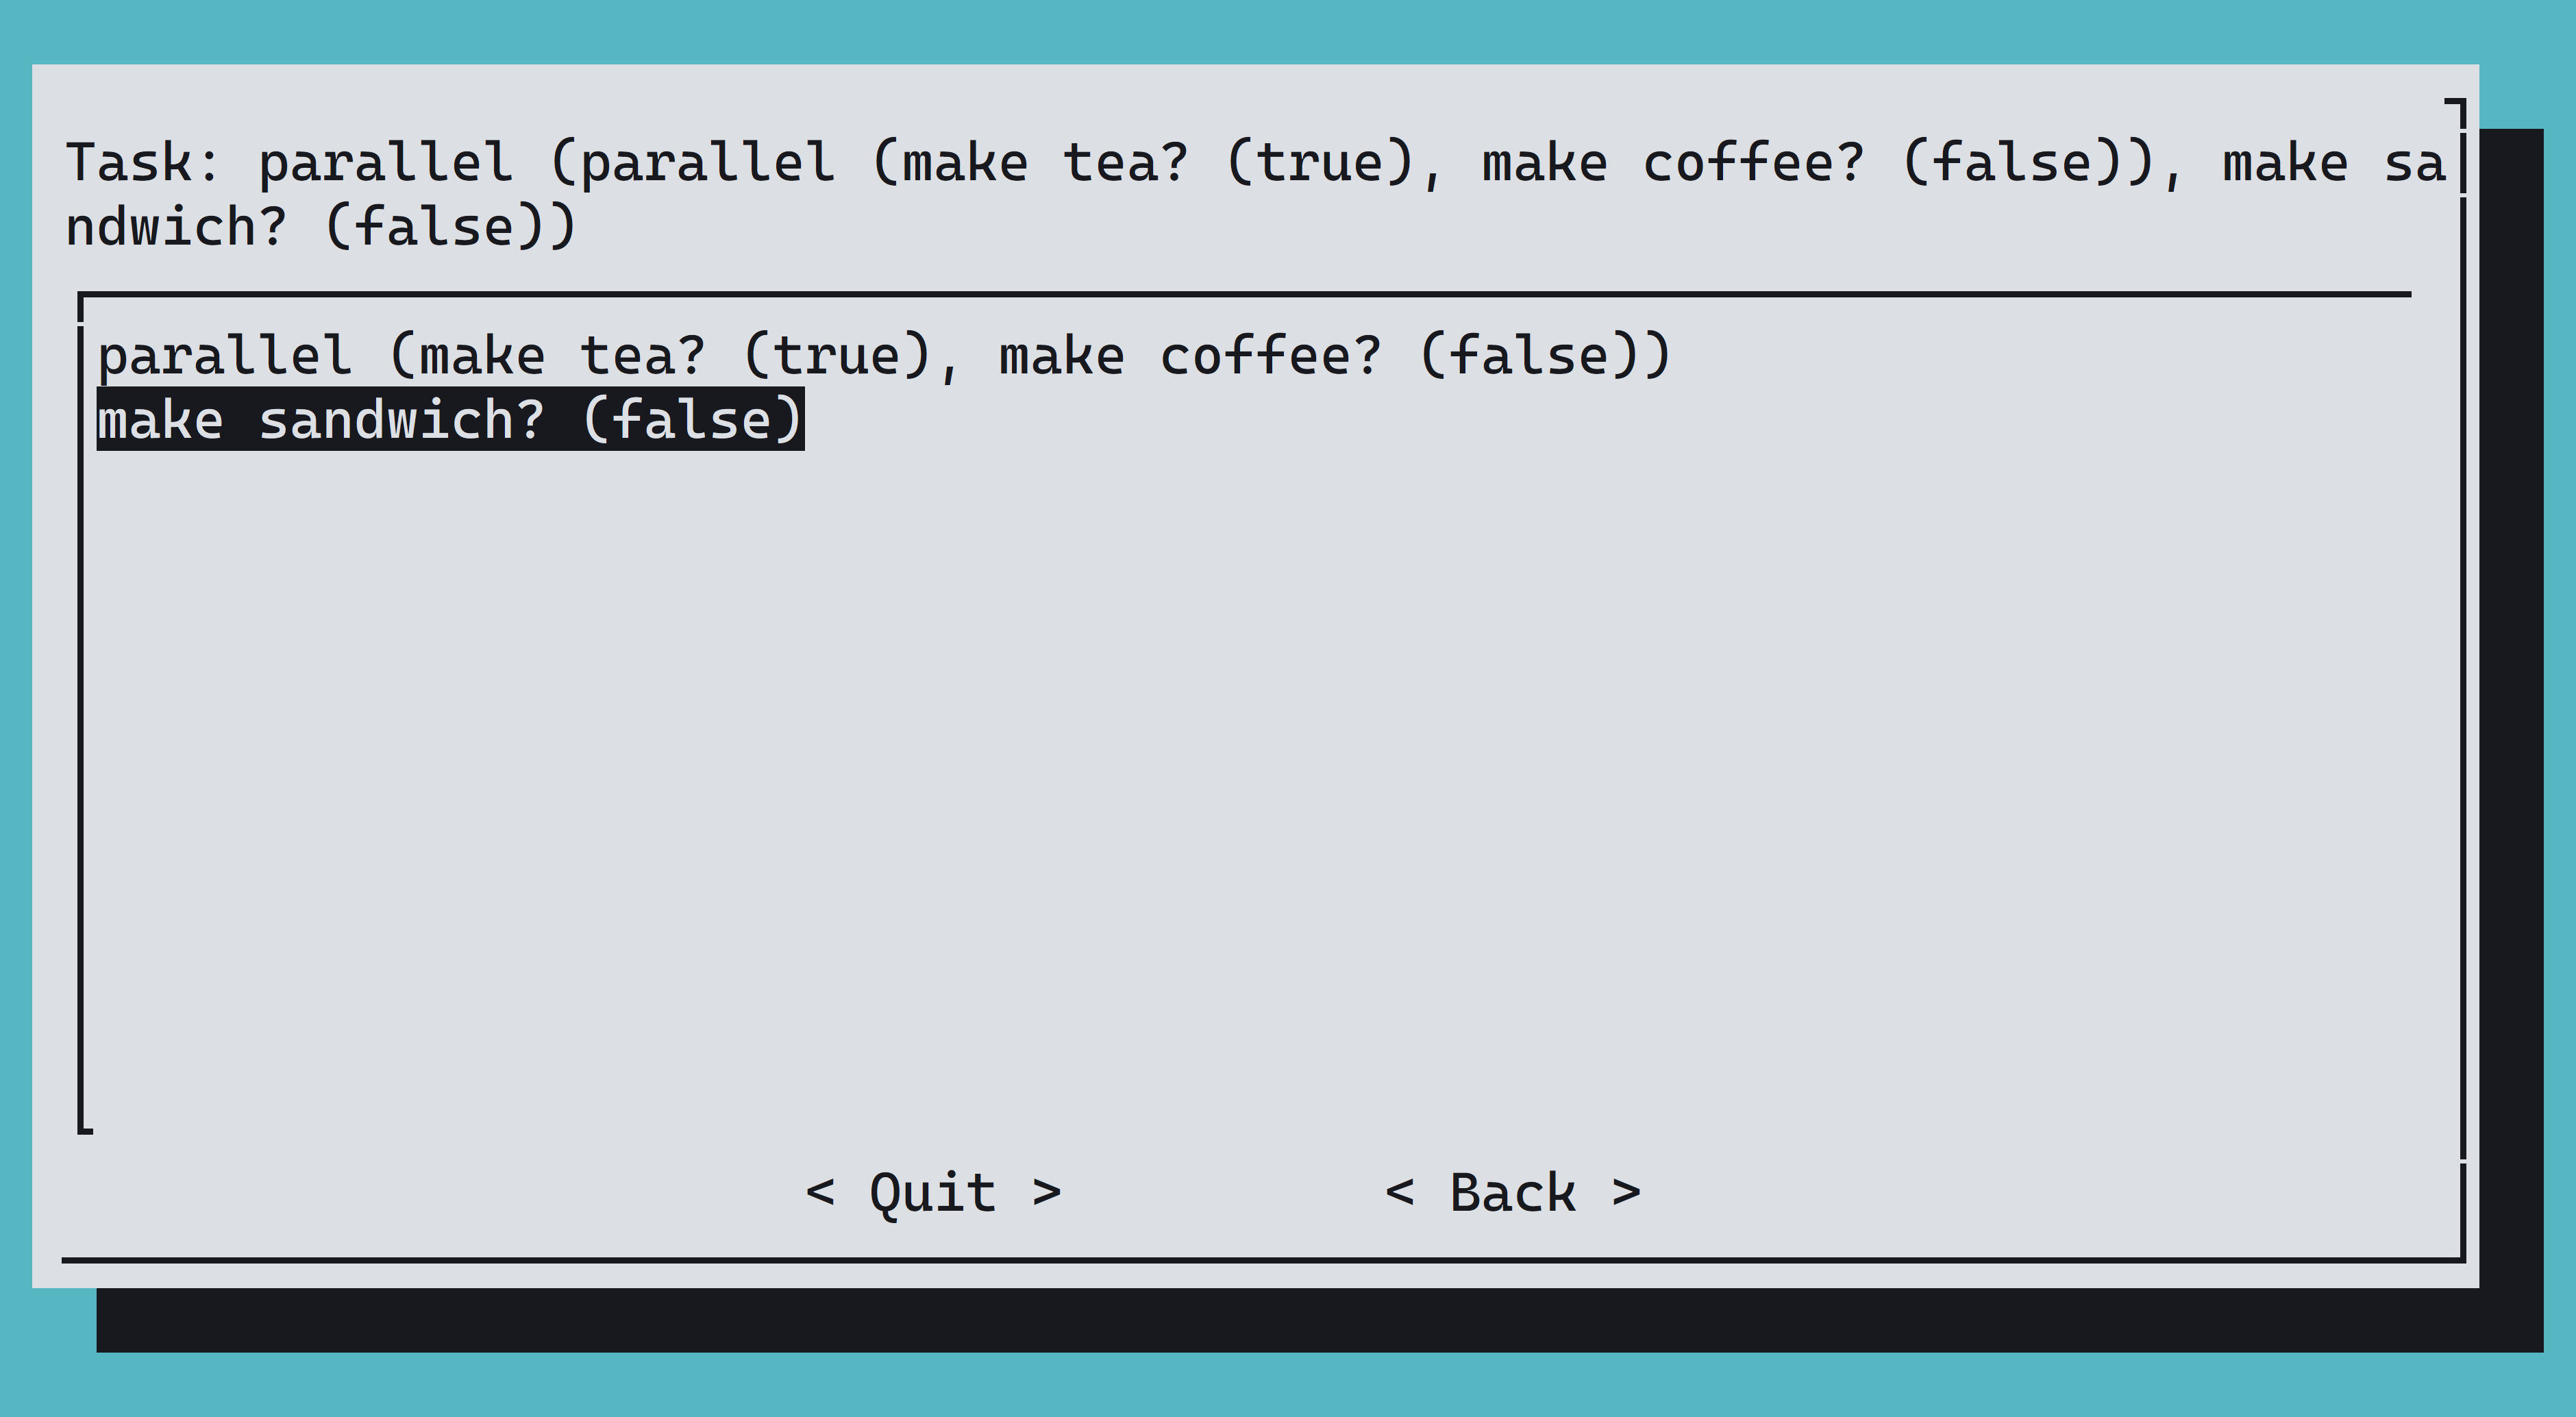
\includegraphics[width=\textwidth]{img/screenshot-ltasks-breakfast.png}
    \caption{The UI showing that \lua{makeTea} is \lua{true} and that \lua{makeCoffee} and \lua{makeSandwich} (selected) are both \lua{false}.}
    \label{fig:comparison_ltask_ui_1}
\end{subfigure}
\begin{subfigure}{0.8\textwidth}
    \centering
    \bigskip
    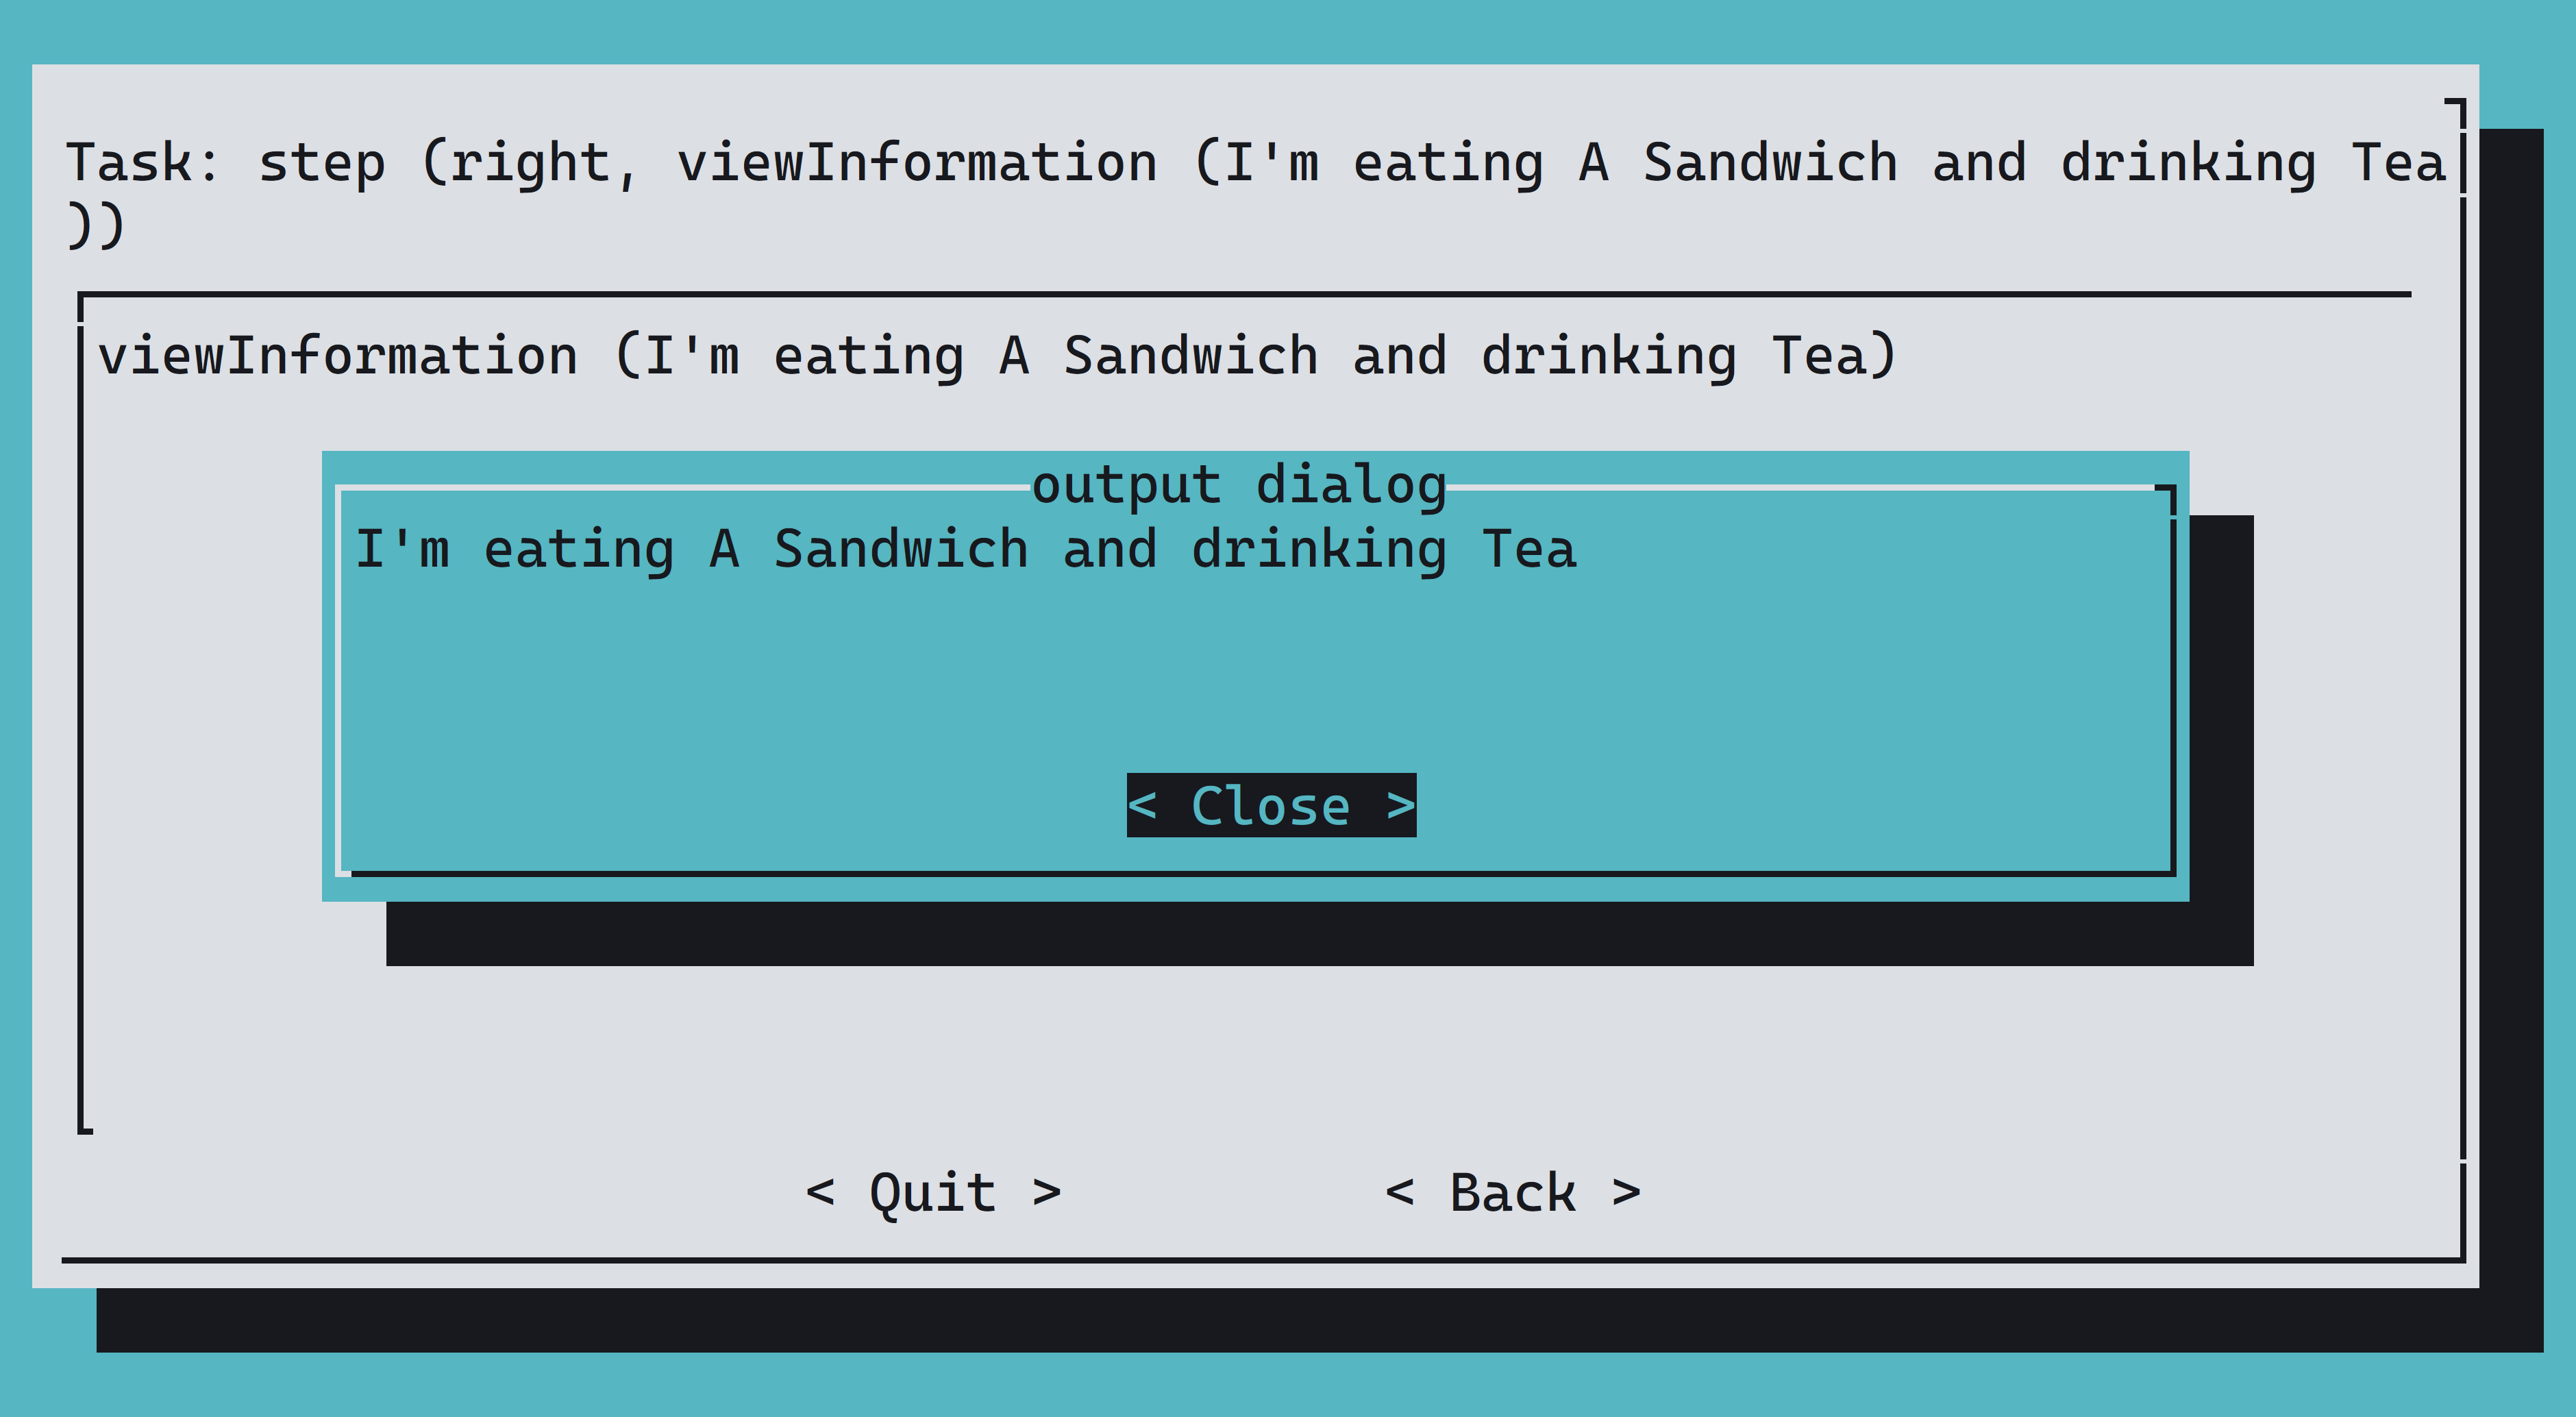
\includegraphics[width=\textwidth]{img/screenshot-ltasks-breakfast-view.png}
    \caption{The UI showing the output after selecting \lua{true} for \lua{makeSandwich}.}
    \label{fig:comparison_ltask_ui_2}
\end{subfigure}
\caption{The textual UI of LTasks.}
\label{fig:comparison_ltask_ui}
\end{figure}

\begin{figure}
\centering
\begin{subfigure}{0.45\textwidth}
    \centering
    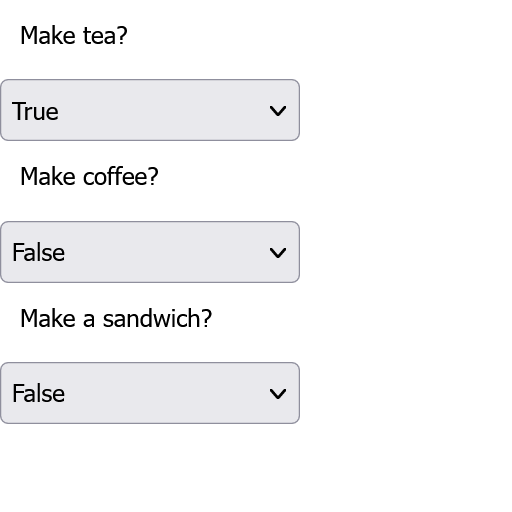
\includegraphics[width=\textwidth]{img/screenshot-itasks-breakfast.png}
    \caption{The UI showing all input fields at once.}
    \label{fig:comparison_itask_ui_1}
\end{subfigure}
\hspace{0.05\textwidth}
\begin{subfigure}{0.45\textwidth}
    \centering
    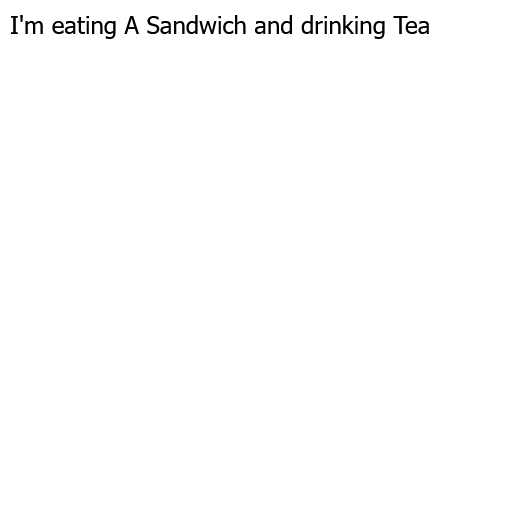
\includegraphics[width=\textwidth]{img/screenshot-itasks-breakfast-view.png}
    \caption{The UI showing the output after selecting \lua{true} for \lua{makeSandwich}.}
    \label{fig:comparison_itask_ui_2}
\end{subfigure}
\caption{The graphical web UI of iTasks.}
\label{fig:comparison_itask_ui}
\end{figure}
